\chapter{Installation} 
\label{chap:install}

We made our implementation open source. The source code can be found in {\it GitHub}. This chapter describes how to install and run our implementation.

\section{Installing Anaconda}

\subsection{Step 1}
To install Anaconda first visit this link- \url{https://www.continuum.io/downloads}.

\subsection{Step 2}
Select your current operating system (Figure \ref{fig:Anaconda1}).
\begin{figure}[!hbt]
\centering

\includegraphics[width=0.8\linewidth]{./img/conda-download1}
\caption{Installing Anaconda: Select Operating System}
\label{fig:Anaconda1}
\end{figure}

\subsection{Step 3}
Download Anaconda for Python 3.XX as shown in Figure \ref{fig:Anaconda1}.
\begin{figure}[!hbt]
\centering
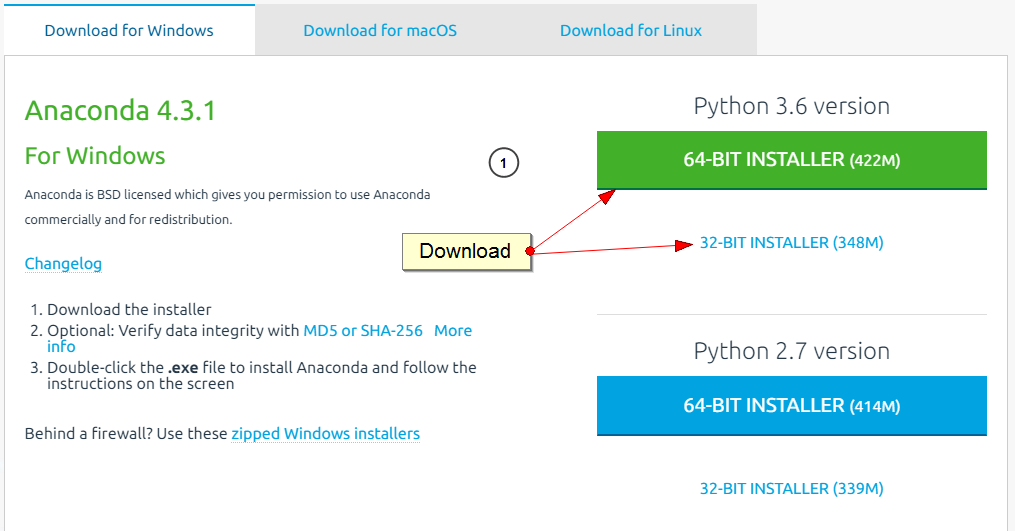
\includegraphics[width=0.8\linewidth]{./img/conda-download2}
\caption{Installing Anaconda: Download for Python 3.XX}
\label{fig:Anaconda1}
\end{figure}

\subsection{Step 4}
After the download is completed, install it. Make sure to set Anaconda directory to you environment variables.
\begin{figure}[!hbt]
\centering
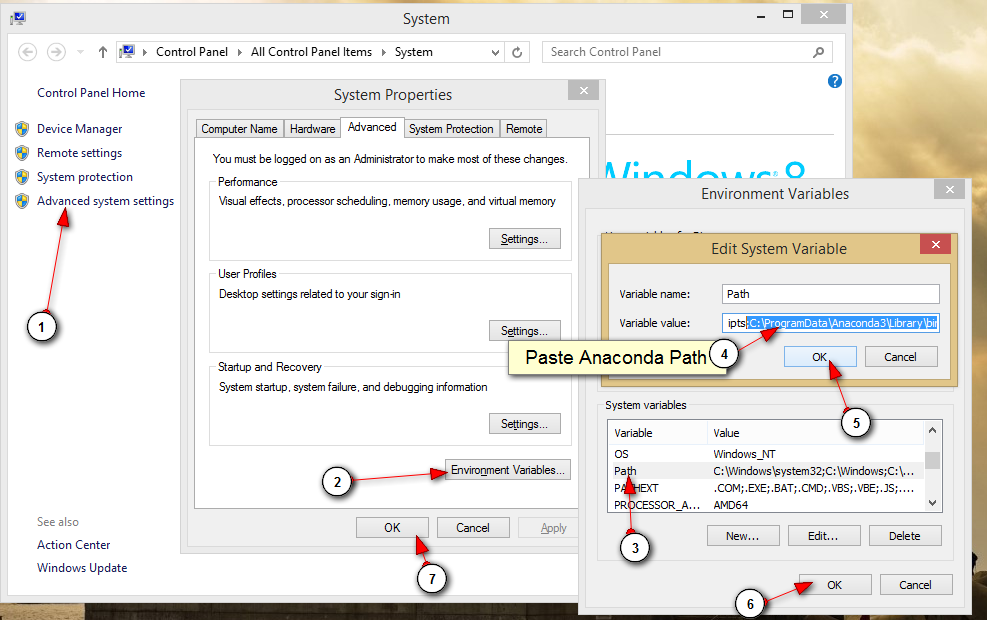
\includegraphics[width=0.8\linewidth]{./img/env-vars}
\caption{Installing Anaconda: Add environment variables (Windows)}
\label{fig:Anaconda1}
\end{figure}

\subsection{Step 4}
Check your installation afterward by typing $conda -V$ and $python --version$ in the Command Prompt. 
\begin{figure}[!hbt]
\centering
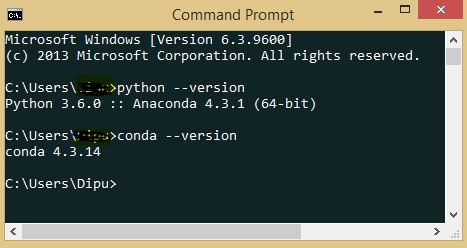
\includegraphics[width=0.8\linewidth]{./img/conda-check}
\caption{Installing Anaconda: Checking installation}
\label{fig:Anaconda1}
\end{figure}


\section{Installing OpenCV} 
Open Command Prompt or Terminal and type: 
\begin{lstlisting}
conda install -c menpo opencv3
\end{lstlisting}. 

If it does not work in Windows system, install using pip: 
\begin{lstlisting}
pip install opencv-python
\end{lstlisting}


\section{Install Git} 
Make sure you have Git installed in your system.
Windows users can install git from \url{https://git-scm.com/downloads}.
Linux users can use apt-get: 
\begin{lstlisting}
sudo apt-get install git
\end{lstlisting}


\section{Clone our repository}
Open the Terminal or Command Prompt and clone the repository using:
\begin{lstlisting}
git clone https://github.com/dipu-bd/alpr-bd
\end{lstlisting}

\section{Usage}
\begin{enumerate}
    \item Create a directory called {\it stages} inside the cloned repository folder.
    \item Save input images inside {\it stages\/stage.0} folder.
    \item Input image file-names should follow the format: {\it <name>.<extension>}. Valid extensions are: JPG, PNG, BMP, and GIF.
\end{enumerate}

\section{Running The Program}
To run the program open terminal or command prompt and type:
\begin{lstlisting}
python .
\end{lstlisting}

It will execute all stages simultaneously. You can however choose individual stage by typing the stage number afterward.
\begin{lstlisting}
python . <stage-number>
\end{lstlisting}

Also, you can execute a range of stages by separating two stage number using minus (-) sign. Here first one is the beginning stage number and last is the end stage number. The program will execute all stages from beginning to end. 
\begin{lstlisting}
python . <from-stage>-<to-stage>
\end{lstlisting}

You can ommit the beginning or the end stage number when declaring a range. To execute all stages from beginning to a specific stage:
\begin{lstlisting}
python . -<to-stage>
\end{lstlisting}

And to execute all stages from a specific stage to very last stage:
\begin{lstlisting}
python . <from-stage>-
\end{lstlisting}

To visit help and available stage numbers type:
\begin{lstlisting}
python . help
\end{lstlisting}


\section{Notes to Developers}
\subsection{Editor choice}
We used **PyCharm** *Community Edition*. You can download it from \url{https://www.jetbrains.com/pycharm/download/}.

\subsection{Definitions}
\begin{description}
    \item[Main.py]: Starting point of the program.
    \item[Stage]: means states of the processing. {\it stage.0} identifies original image list.
 After applying first step the `stage.1` is found, and so on.
    \item[alpr.py]: It connects all functions with stage numbers.    
\end{description}

\subsection{Stage Artifacts}
\begin{itemize}
    \item {\bf Stage Artifacts} are the output files generated after executing each stages.
    \item The output images should be stored inside {\it stage.<stage\_number>} folder.
    \item The format of these image file: {\it <name>.<extension>}. 
    \item Here {\it <name>} refers to the name of original image.
\end{itemize}

\subsection{Creating A Stage}
\begin{enumerate}
    \item Create a python file inside {\it modules} folder. 
    \item Import it inside {\it alpr.py}.
    \item Insert the name of the function in {\it STAGE\_FUNC} variable.
\end{enumerate}

